\documentclass[UTF8]{ctexbeamer}	% Compile at least twice!
%\setbeamertemplate{navigation symbols}{}
\usetheme{Berlin}
% \useinnertheme{rectangles}
\useoutertheme{infolines}
\useoutertheme[title,section,subsection=true]{smoothbars}
% \useoutertheme{split}
\useinnertheme{rounded}
\usecolortheme{default}
% \usecolortheme{whale}
 
% -------------------
% Packages
% -------------------
\usepackage{
    amsmath,			% Math Environments
    amssymb,			% Extended Symbols
    enumerate,		    % Enumerate Environments
    graphicx,			% Include Images
    lastpage,			% Reference Lastpage
    multicol,			% Use Multi-columns
    multirow,			% Use Multi-rows
    pifont,			    % For Checkmarks
    stmaryrd,            % For brackets
    listings,
}
\usepackage[english]{babel}
\usepackage{graphicx}
% \usepackage{CJK}
\lstset{language=C++}
\lstset{extendedchars=false}
\lstset{breaklines}


% -------------------
% Colors
% -------------------
% \definecolor{UniOrange}{RGB}{212,69,0}
% \definecolor{UniGray}{RGB}{62,61,60}
% \definecolor{UniRed}{HTML}{B31B1B}
% \definecolor{UniGray}{HTML}{222222}
% \setbeamercolor{title}{fg=UniGray}
% \setbeamercolor{frametitle}{fg=UniOrange}
% \setbeamercolor{structure}{fg=UniOrange}
% \setbeamercolor{section in head/foot}{bg=UniGray}
% \setbeamercolor{author in head/foot}{bg=UniGray}
% \setbeamercolor{date in head/foot}{fg=UniGray}
% \setbeamercolor{structure}{fg=UniOrange}
% \setbeamercolor{local structure}{fg=black}
% \beamersetuncovermixins{\opaqueness<1>{0}}{\opaqueness<2->{15}}


% -------------------
% Fonts & Layout
% -------------------
\useinnertheme{default}
\usefonttheme{serif}
\usepackage{palatino}
\setbeamerfont{title like}{shape=\scshape}
\setbeamerfont{frametitle}{shape=\scshape}
\setbeamertemplate{itemize items}[circle]
%\setbeamertemplate{enumerate items}[default]


% -------------------
% Commands
% -------------------

% Special Characters
\newcommand{\N}{\mathbb{N}}
\newcommand{\Z}{\mathbb{Z}}
\newcommand{\Q}{\mathbb{Q}}
\newcommand{\R}{\mathbb{R}}
%\newcommand{\C}{\mathbb{C}}

% Math Operators
\DeclareMathOperator{\im}{im}
\DeclareMathOperator{\Span}{span}

% Special Commands
\newcommand{\pf}{\noindent\emph{Proof. }}
\newcommand{\ds}{\displaystyle}
\newcommand{\defeq}{\stackrel{\text{def}}{=}}
\newcommand{\ov}[1]{\overline{#1}}
\newcommand{\ma}[1]{\stackrel{#1}{\longrightarrow}}
\newcommand{\twomatrix}[4]{\begin{pmatrix} #1 & #2 \ #3 & #4 \end{pmatrix}}


% -------------------
% Tikz & PGF
% -------------------
\usepackage{tikz}
\usepackage{tikz-cd}
\usetikzlibrary{
    calc,
    decorations.pathmorphing,
    matrix,arrows,
    positioning,
    shapes.geometric
}
\usepackage{pgfplots}
\pgfplotsset{compat=newest}

\usepackage{wrapfig}
\usepackage{cite}


% -------------------
% Theorem Environments
% -------------------
\theoremstyle{plain}
\newtheorem{sit}{Situation}[section]
\newtheorem{prop}{Proposition}[section]
\newtheorem{rtm}{Theorem}[section]
\newtheorem{cor}{Corollary}[section]
\theoremstyle{definition}
\newtheorem{das}{Data structure}[section]
\newtheorem{nex}{Non-Example}[section]
\newtheorem{cla}{class}[section]
\newtheorem{emt}{}[section]
\newtheorem{defn}{Definition}[section]
\theoremstyle{remark}
\newtheorem{rem}{Remark}[section] 
\numberwithin{equation}{section}

\newcommand\caesura{$\mkern -8.5mu\raise -.2ex\hbox{\rotatebox[]{180}{\`}}\ $}

% -------------------
% Title Page
% -------------------
\title{\textcolor{white}{2021年秋季入学硕博连读综合面试报告}}
%\subtitle{\textcolor{white}{Mathematics Conference for the Mysterious and dMagical}}  
\author{谭焱(张庆海)}
\institute{浙江大学数学科学学院}
\date{\today} 


% -------------------
% Content
% -------------------
\begin{document}
% \begin{CJK}{GBK}{kai}

% Title Page
\begin{frame}
\titlepage
\end{frame}



% Motivation
\section{个人基本情况介绍}


% \begin{frame}
%     \begin{emt}[过往受教育经历]
%         \begin{enumerate}
%             \item 高中在湖南师范大学附属中学就读时参与数学奥林匹克竞赛.
%         \end{enumerate}
        
%     \end{emt}
% \end{frame}


% Definitions & Examples
\begin{frame}[fragile]
    \begin{emt}[个人学习经历]
\begin{enumerate}
    \item 高中在湖南师大附中就读时参与数学奥林匹克竞赛.
    \begin{itemize}
        \item 高二高三两年获得数学竞赛省一等奖.
    \end{itemize}
    \item 研究生课程学分修读情况
    \begin{itemize}
        \item 已修满硕士学位要求的学分,并在与我的科研项目相关的部分课程中取得良好成绩.
        \begin{itemize}
            \item 非线性问题的数学方法(92), 图形学的新进展(90) 等.
        \end{itemize}
        \item 英语阅读及写作方面
        \begin{itemize}
            \item 六级489分(阅读205)可以流畅阅读英文文献.
            \item 通过课程研究生论文写作指导(92)打下坚实写作基础.
        \end{itemize}
    \end{itemize}
\end{enumerate}
\end{emt}
\end{frame}

\begin{frame}[fragile]
   \begin{emt} [研究项目参与情况]
    \begin{enumerate}
        \item 2019年春学期,独立完成程序.实现张老师的论文中的二维空间内殷集上的布尔代数.
        为之后的三维空间内殷集之间的布尔代数的研究做好铺垫.
        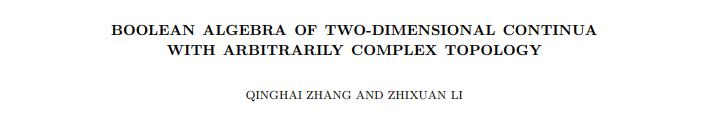
\includegraphics[width = \linewidth]{fig/articlename1.png}
        \item 2020年秋学期,在张老师的指导下,和学长合作研究微地震反问题.最终得到一个能根据
        检波器接收到的地震波信号输出合理的震源位置的程序.
        \item 2021年春学期,与学弟分工推进三维殷集的表示,及通过编程实现在计算机上计算
        三维殷集之间的布尔运算.
    \end{enumerate}
   \end{emt}
\end{frame}

\section{研究生项目详细介绍}
\subsection{微地震的反问题}

\begin{frame}
    \frametitle{微地震探测反问题研究}
    \begin{itemize}
        \setlength{\itemsep}{30pt}
        \item \textbf{背景 : } 项目的意义和要做的问题.
        \item  \textbf{解决过程 : } 切分问题,分步实现.
        \item \textbf{实现结果 : } 对真实数据计算结果图和总结.
    \end{itemize}
\end{frame}

\begin{frame}
    \begin{emt}[背景及意义]
      
    \begin{itemize}
        \begin{columns}
            \column{0.8\linewidth}<1->
    % \begin{wrapfigure}[r]{5cm}
    %    \centering
       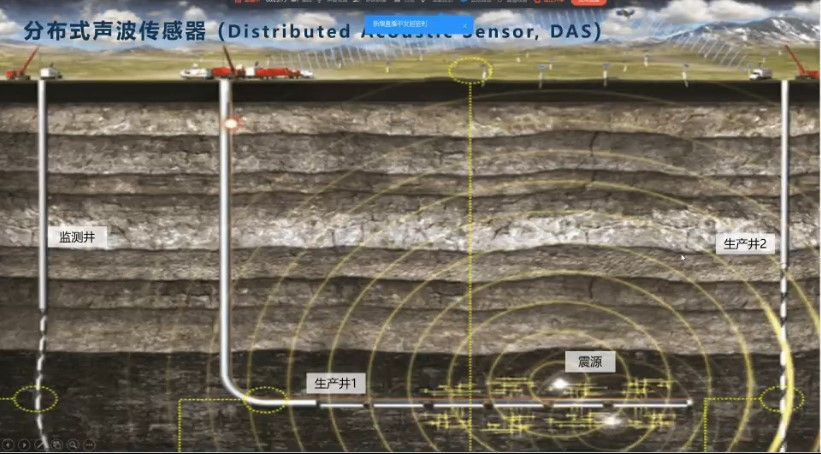
\includegraphics[width = \textwidth]{fig/s2p1.jpg}
    %    \caption{\footnote{ 油气田中的生产井和监测井}}
    % \end{wrapfigure}
    \column{0.2\linewidth}<1->
    \item  微地震通常是由于地质勘探或者一些开采活动导致地下裂缝错位,从而形成的
低频率弹性波.\cite{wu_1991}
\end{columns}
\item 作为一种人为产生的地震,其产生的信号经常出现于石油天然气工程作业.
近些年来,国际上众多的研究机构与微震公司已经证明了微地震监测方法在油气田
规划与开发方面的指导意义.

    \end{itemize}

    
\end{emt}
\end{frame}

\begin{frame}

  \begin{emt}[要解决的问题]
    \begin{itemize}
        \item \textbf{输入: }
        \begin{itemize}
            \item 监测井附近的地质信息
            % (包含地震波在各个地层的理论传播速度及地层结构).
            \item 每个检波器收到的地震波信号的时间和检波器的位置.
        \end{itemize} 
        \item \textbf{输出: } 
        \begin{itemize}
            \item 接收到的微地震信号对应的震源位置. 
        \end{itemize}
    \end{itemize}

    \begin{emt}[问题的难点]
        \begin{enumerate}
            \item 地震波在不同速度的地层中传播不是沿直线传播.
            % 复杂的地层信息使得检波器的地震波到时与震源位置之间是强非线性关系.

            \item 因为微地震的震级小的原因,通常只有部分检波器能接收到合理的地震波到时信息.
            
        \end{enumerate}
        
    \end{emt}
      
  \end{emt}
\end{frame}



% Main Results



% Theorem
\begin{frame}
  \begin{emt}[将总的问题切分为几部分]
    \begin{enumerate}
        \item 从已有的地层信息建立分片函数拟合两个相邻地层之间的界面.
        \item 假设地震波在地层内部匀速直线传播,在穿过相邻地层之间的界面时发生折射.
        求解地震波从假设震源到每个检波器的传播路径.
        \item 
        % 已知地震波的传播路径可以得到每个检波器理论接收到地震波的相对到时.
        根据每个检波器的真实接受地震波的相对到时和理论值建立残差方程.
        \item 对残差方程近似求解得到使残差值最小的震源位置.
    \end{enumerate}
  \end{emt}
\end{frame}

\begin{frame}
  \begin{emt}[拟合地震波发生折射的界面]
    \begin{itemize}
        \item \textbf{输入 : } 标记相邻地层分界面的点集.
        \item \textbf{输出 : } 表示相邻地层分界面的分片曲面
    \end{itemize}
    
    \begin{columns}
        \column{0.4\linewidth}<1->
        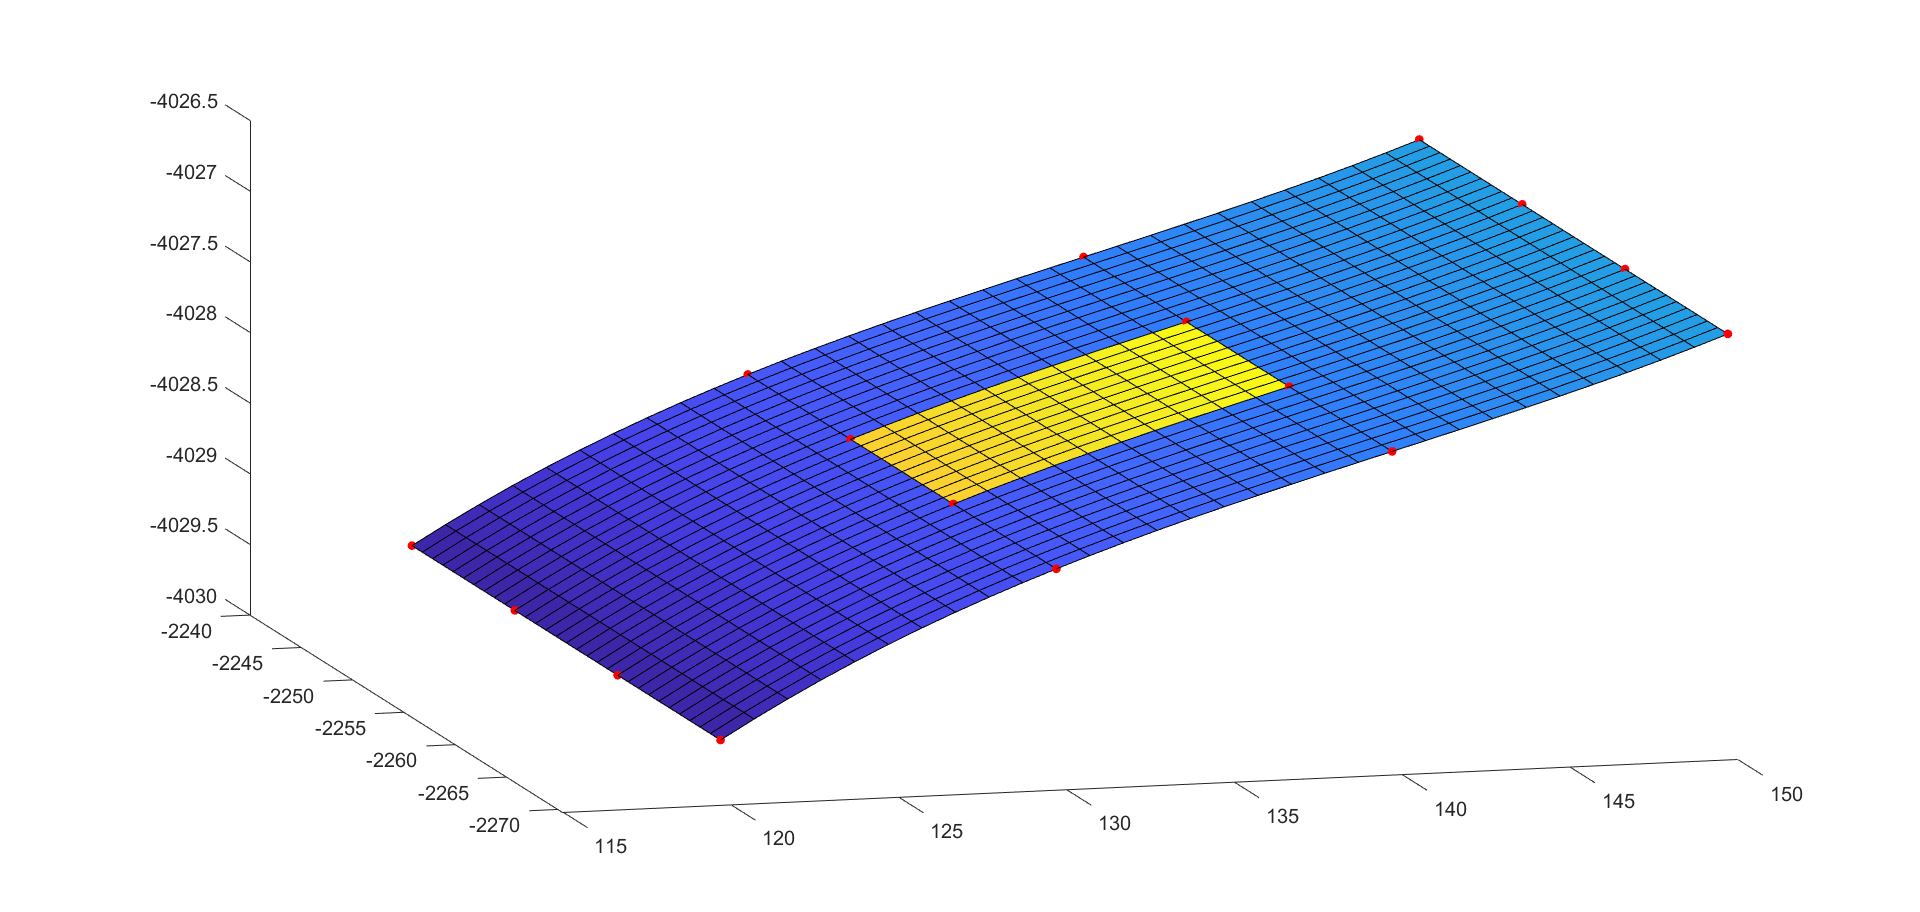
\includegraphics[width = \textwidth]{fig/s2p2.png}
        \column{0.6\linewidth}<1->
        \begin{itemize}
        \item 如图所示, 其上的红色点是输入的点集.选取12个点建立12个方程.
        \item 方程组最小二乘拟合得到三维坐标的z值关于x,y二元三次函数(图中蓝色部分),
        \item 限制函数的定义域得到一片区域上的地层分界面拟合(黄色区域).
        % 合并所有局部函数得到表示整个地层分界面的分片曲面.
        \end{itemize}
    \end{columns}

      
  \end{emt}
\end{frame}





% Corollary
%\begin{frame}

%\begin{cor}
%For all n,m \in \N$, $(n+m)^2= n^2 + m^2$.
%\end{cor}
%\end{frame}







% Application 1
\begin{frame}[fragile]
 \begin{emt}[地震波传播路径求解]
    \begin{itemize}
        \item \textbf{输入 : } 地质模型,检波器和假设震源的坐标.
        \item \textbf{输出 : } 地震波从震源传播到检波器的路径.
    \end{itemize}
 \end{emt}

 \begin{defn}[Fermat's principle]
    光传播的路径是光程取极值的路径.
 \end{defn}

 \begin{emt}[转化为数学问题]
    \begin{itemize}
        \item 不妨设起始点和终点分别为$(x_0,y_0,z_0),(x_1,y_1,z_1)$,两个地层中地震波传播速度为$v_0,v_1$.
        传播时间函数$f(x,y)$如下定义
        \begin{tiny}
         \begin{equation}
            f(x,y) = \sqrt{(x - x_0)^2 + (y - y_0)^2 + (z(x,y) - z_0)^2} / v_0 + 
            \sqrt{(x - x_1)^2 + (y - y_1)^2 + (z(x,y) - z_1)^2} / v_1.
        \end{equation}
    \end{tiny}
        % 上式为地震波从起点传播到终点的时间关于地震波在地层分界面上的折射点$(x,y,z(x,y))$的函数
        % $f(x,y)$.
    \end{itemize}
     
 \end{emt}
\end{frame}






% Math
\begin{frame}
  \begin{emt}[牛顿迭代求解]
      \begin{itemize}
          \item 
        %   因为$z$关于$x,y$的函数就是之前拟合的分片三次函数,因此$z$有关于
        %   $x,y$的分片连续二阶导数.所以可以通过
          对$f$求导的牛顿迭代法计算得到使得地震波传播时间最短的折射点.

          \item 对于多个地层多个折射点的情况,固定其他折射点,每次迭代求解一个折射点.
          循环多次得到所有的折射点位置使得地震波传播时间最短的路径.

          \item 对于一个假设震源和两个检波器,迭代得到的传播路径如下图
          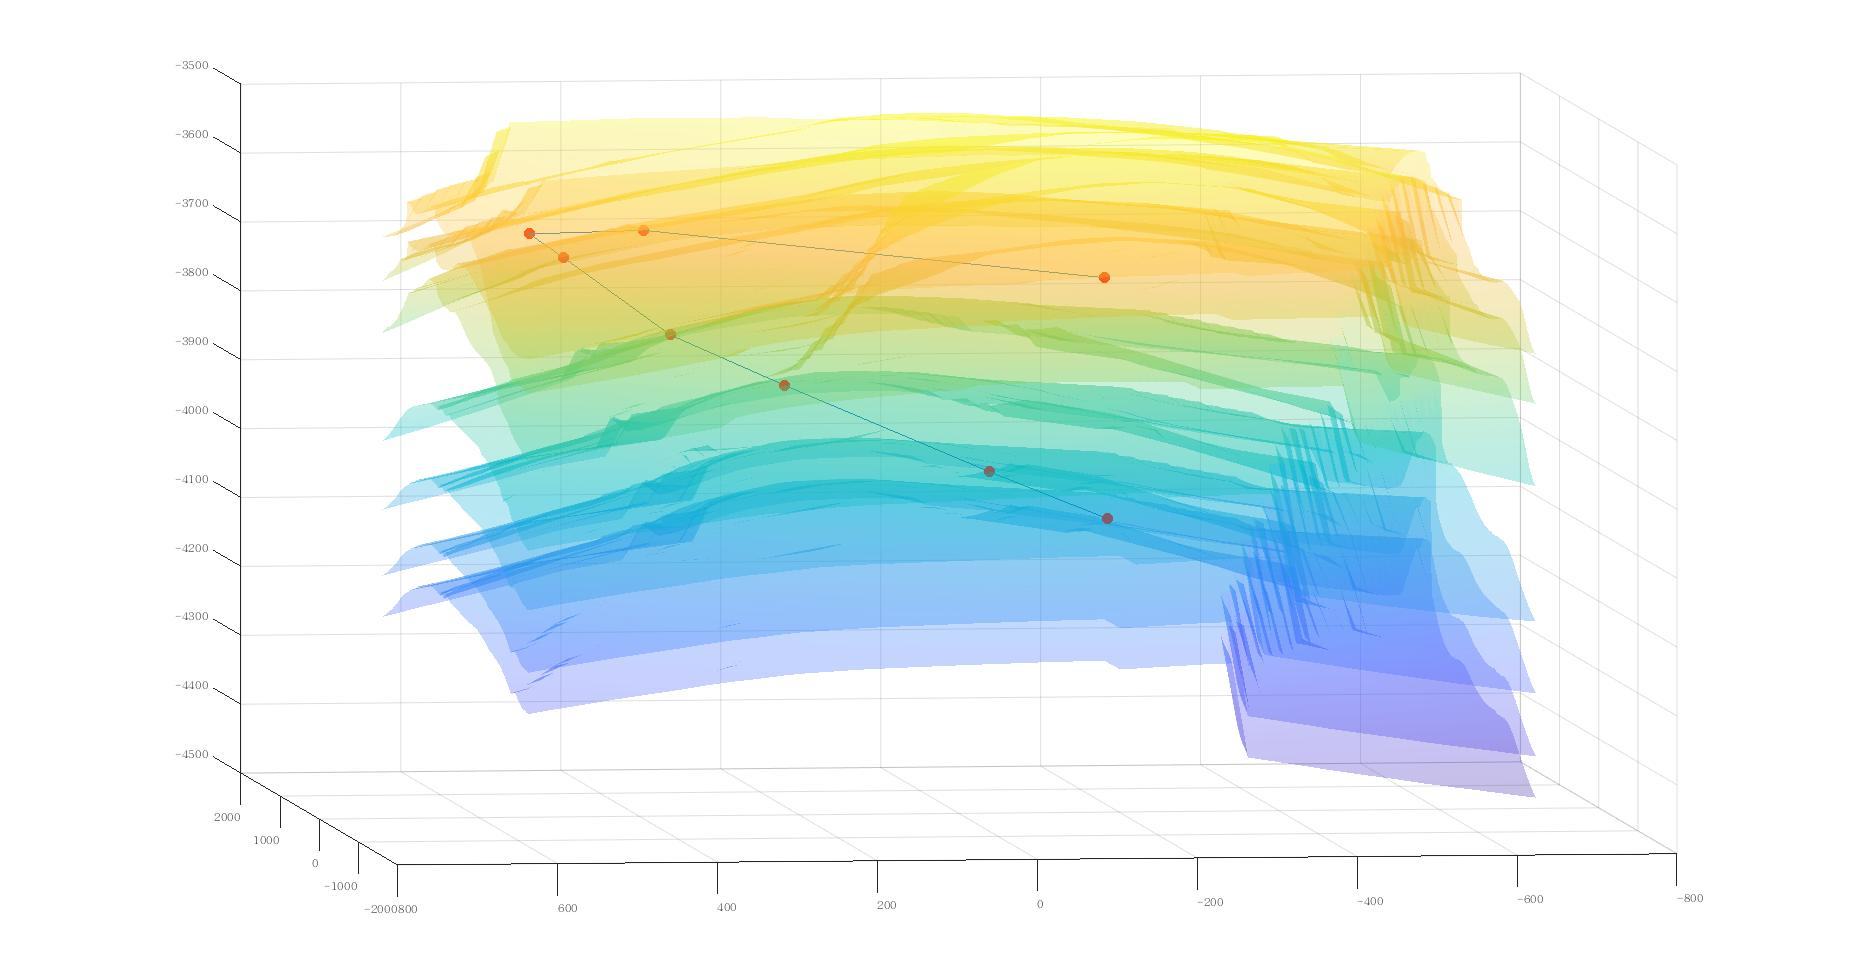
\includegraphics[width = .6\textwidth]{fig/s2p4.jpg}
      \end{itemize}
  \end{emt}
\end{frame}

\begin{frame}
\begin{emt}[残差方程组]
    \begin{itemize}
        \item 当震源和检波器位置确定时,定义地震波传播路径的长度$D_i$,
        结合已有的各个地层中地震波传播速度计算可得传播时间$T_i$.
        \item 现实中接收到地震波信号的时间不妨设为$T_i^\prime$.
        \item 定义残差方程组如下
        \begin{small}
            \begin{equation}
                Res_{ij} = D_i * D_j(\frac{1}{T_j} - \frac{1}{T_i}) + \frac{D_i * D_j}{T_i * T_j}((T_i - T_j) 
                 - (T_i^\prime - T_j^\prime)).
            \end{equation}
        \end{small}
    \end{itemize}
\end{emt}
\end{frame}






% End Slide
\begin{frame}
    \begin{emt}[残差方程组求解]
        \begin{enumerate}
            \item 求解残差方程组第一种方法是对残差关于震源坐标的函数迭代求解.当接收到
            地震波信号的检波器数量较多时,可以采取这个方法.
            \begin{itemize}
                \item 将关于震源坐标求导的过程转化为差分形式.
                \item 在迭代过程中加入模拟退火等防止陷入局部解的方法.
            \end{itemize}

            \item 
            % 但是,微地震是一种能量非常小的地震.通常情况由于接收到信号的检波器太少,
            % 距离太接近会导致残差方程组的求解过程条件数过大.并且由于检波器都在一条几乎
            % 直线的检测井内,震源的x,y坐标也难以计算.
            当接受到地震波信号的检波器数量过少时,我们使用检索的方式.

            \begin{itemize}
                \item 预先在监测井附近的空间上均匀选取样本点.计算每个样本点作为震源时
                所有检波器接收到地震波信号的理论时间.

                \item 当实际接收到地震波信号时,使用预先计算好的理论到时计算每个样本点
                关于实际接收信号的到时的残差值,输出使得残差较小的样本点集合.

                \item 根据微地震形成原理,一般发生在地层断层附近,筛选输出的样本点.
                % 集合和断层位置比对,输出合理的震源估计.
            \end{itemize}
        \end{enumerate}
    \end{emt}
\end{frame}



% Questions
\begin{frame}
\begin{emt}[几个月的实际数据计算结果]
    \begin{columns}
        \column{0.4\linewidth}<1->
        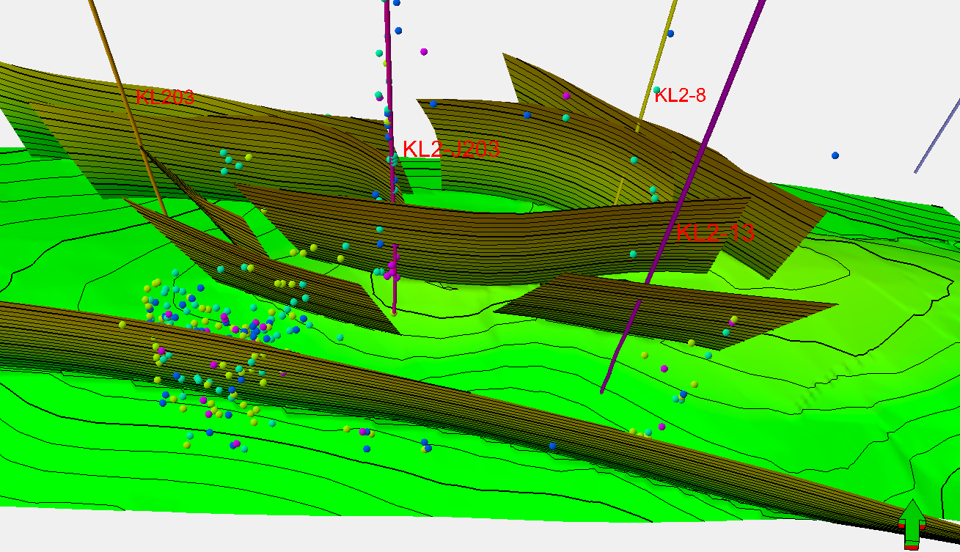
\includegraphics[width = \textwidth]{fig/s2p5.png}
        \column{0.4\linewidth}<1->
        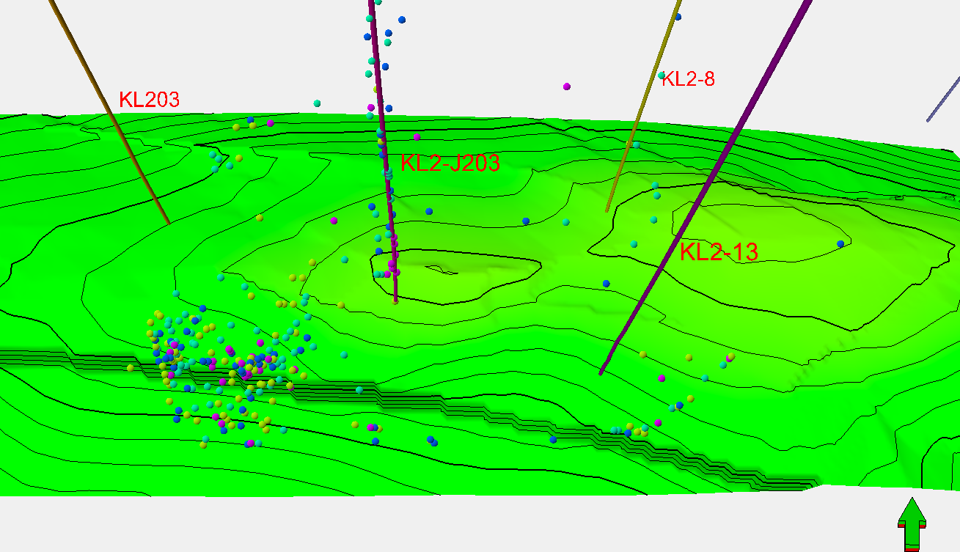
\includegraphics[width = \textwidth]{fig/s2p6.png}
    \end{columns}

    \begin{itemize}
        \item 两幅图中都可以看出微地震多发生在断层附近.
        \item 由于对于一条直线上的检波器,以该直线为中心的圆周上的地震事件,检波器接收
        的地震波信号几乎一样,所以能在输出的震源中看出圆弧形状.
    \end{itemize}
\end{emt}
\end{frame}

\subsection{三维殷集上的布尔代数}

\begin{frame}
    \frametitle{三维殷集模型和殷集上的布尔代数}
    \begin{itemize}
        \setlength{\itemsep}{30pt}
        \item \textbf{背景 : } 需要解决的问题,和问题的意义.
        \item \textbf{模型实现 : } 推导理论的同时,将数学结构使用数据结构实现.
        \item  \textbf{部分结果 : } 部分测试结果.
    \end{itemize}
\end{frame}

\begin{frame}
    \begin{emt}[背景与意义\cite{2020Boolean}]
        \begin{itemize}
            \item 均匀连续的有物理意义的区域是普遍存在的,对其建模在无数科学和工程应用中具有重要意义.
            \item 
            % 在二维和三维空间中,对物理区域建模是被称为实体建模的成熟的研究课题.但是在
            在多相流领域中,一直在避免对流体建模.但是随着随着多相流研究的迅速发展,
            需要建立这样一个流体模型,以便对复杂的现象,如涉及流体拓扑变化的现象,进行严格的研究.
            \item 为了回答建模空间上的问题,在建模空间中执行的操作必不可少.
            我们实现的操作是在有任意拓扑复形结构的物理区域上的布尔运算.
            \item 张老师及学长已完成二维空间上的建模和布尔运算的证明,并且提供了高效的代码实现.
        \end{itemize}
    \end{emt}
\end{frame}

\begin{frame}
    \begin{emt}[建模]
        \begin{itemize}
        \item 定义三维殷集$Y$表示三维空间中有物理意义的区域.
         \begin{defn}
             一个殷集$Y \subset \mathbb{R}^3$是一个边界有界的规则半解析开集.所有的这样的殷集
             集合构成殷集空间$\mathbb{Y}$.
         \end{defn}
        \begin{cor}
            殷集边界$\partial Y$上的点$p$满足,对点$p$充分小的邻域$N(p)$,
        \begin{itemize}
            \item $\partial Y \cap N(p)$是有限个广义圆盘的并集.
            \item 上一条中的圆盘仅在有限条广义半径相交,广义半径端点都在$N(p)$上,且两两之间
            仅相交于点$p$.
            \item 半径将圆盘切分为广义扇形的集合,$N(p) - \partial Y$被$\partial Y$划分为有限个
            不相交的规则开集.对于两个有扇形作为公共边界的开集,其中一个属于殷集内部,另一个属于
            外部.
        \end{itemize}
        \end{cor} 
        \end{itemize}
    \end{emt}
\end{frame}

\begin{frame}
    \begin{emt}[曲面片]
        为了使用计算机计算殷集上的布尔运算,需要建立数据结构保存殷集的空间结构.
        \begin{itemize}
            \item 由推论中殷集边界上的点的性质可知,
            主要关注$N(p) \cap \partial Y$超过一个圆盘的点p.
            \item 所以使用曲面片作为表示殷集边界的基本元, 曲面片内部点是领域只包含一个圆盘
            的平凡情况,而边界是所有奇异点.
            % 转化为程序中的体现为,表示殷集边界的基础结构为有边界的曲面片.曲面片内的点
            % 包含了所有邻域内只有一个圆盘的平凡情况,边界上的点是邻域内超过一个圆盘的特殊点.
        \end{itemize}
        目前对于曲面片的边界定义不够准确.结合如下推论
        \begin{cor}
三维空间中的殷集$Y$满足
\begin{itemize}
    \item $\partial Y$包含有限个孤立奇异点.
    \item $\partial Y$中的非孤立奇异点构成一个紧的一维CW复形.
\end{itemize}
            \end{cor}
            所以在忽略所有孤立奇异点的情况下,曲面片的边界是一维曲线的集合.
    \end{emt}
\end{frame}

\begin{frame}
    \begin{emt}[曲面片]
        % 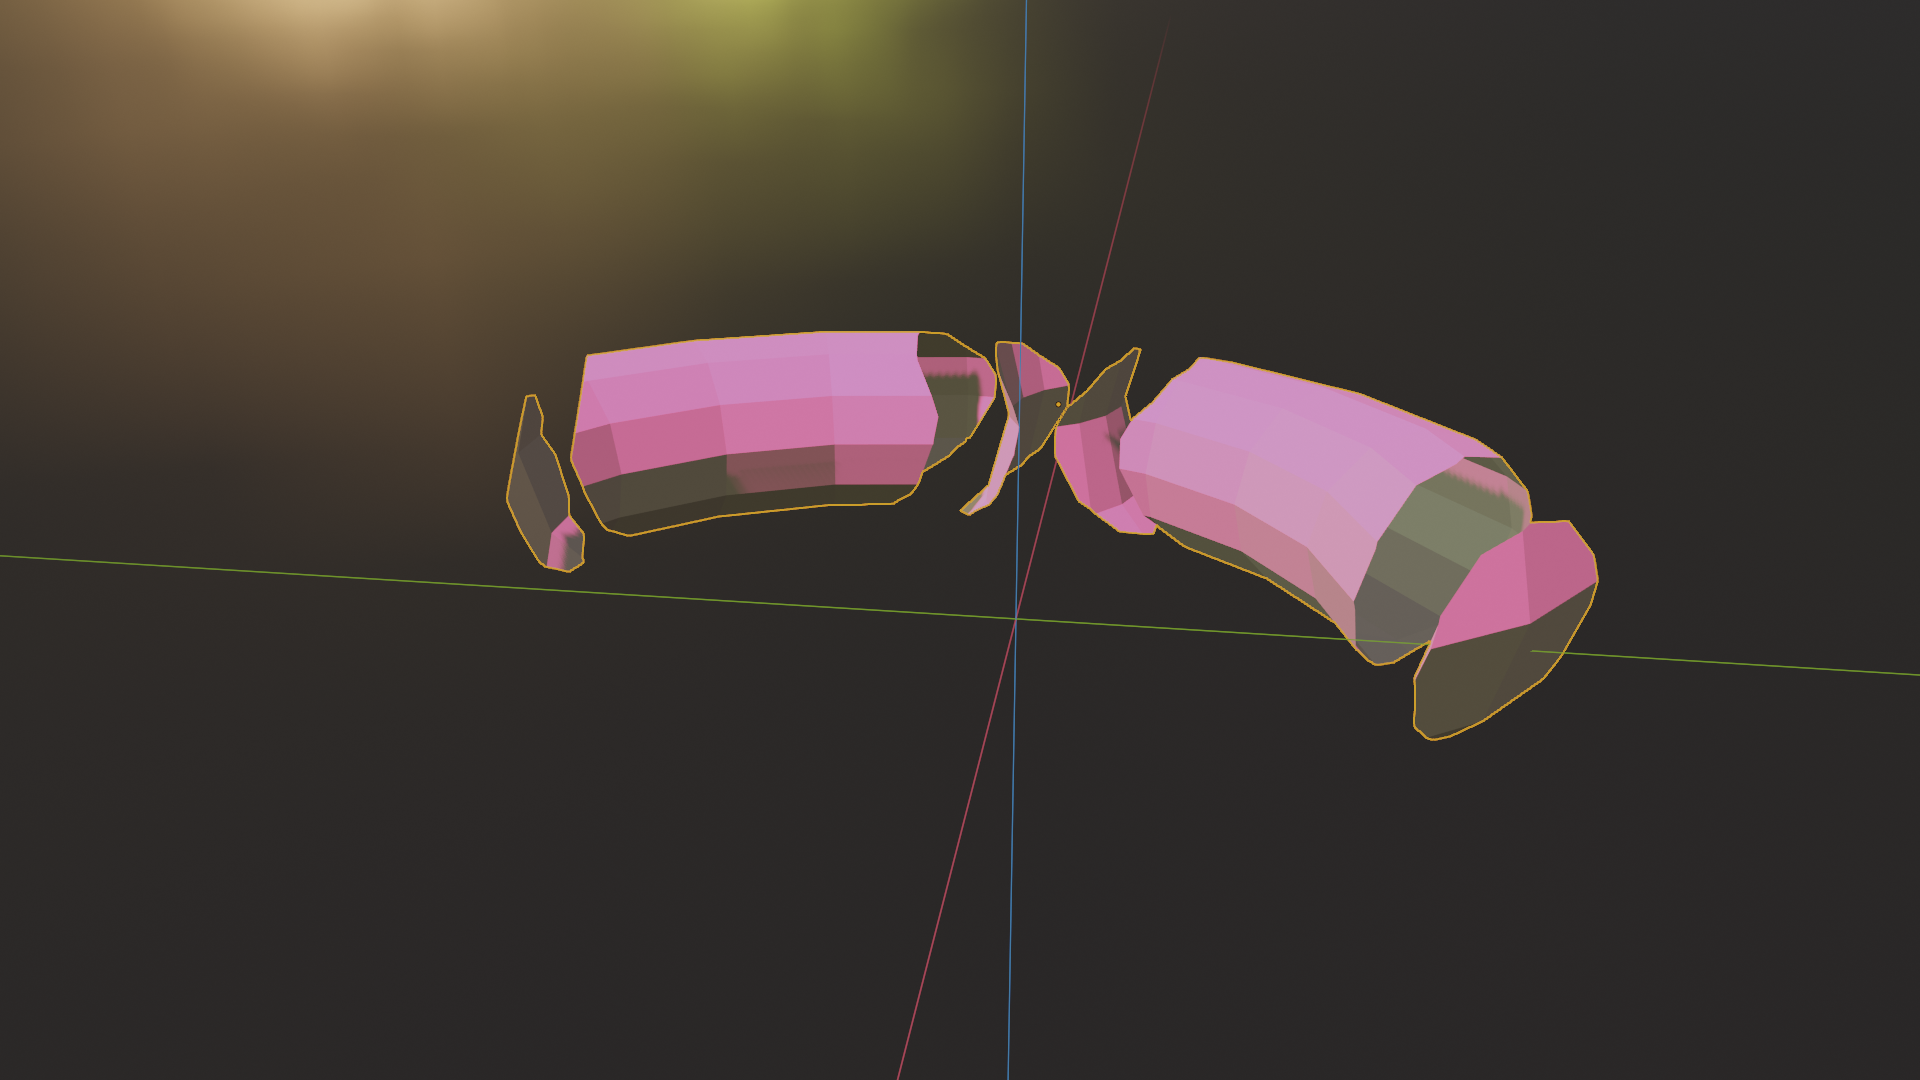
\includegraphics[width = \textwidth]{fig/s3p1.png}
    \end{emt}
\end{frame}

\begin{frame}
    \begin{emt}[黏合紧曲面]
        只有曲面片不能唯一表示殷集边界$\partial Y$.所以需要找到合适的方法将曲面片
        沿它们的边界粘合起来作为殷集的唯一表示.我们引入黏合紧曲面的定义.

        \begin{defn}
            黏合紧曲面是一个二维连通紧流形或这种流形的一个商空间,其商映射将多个与
            一维CW复形同胚的子集粘在一起;将这个一维子集删除后该黏合紧曲面仍然是连通的.
        \end{defn}

        并且证明了
\begin{rtm}
    $\partial Y$同胚于将一个集合中的黏合紧曲面沿着同胚于一维CW复形的子集粘起来的结果.
\end{rtm}

    \end{emt}
\end{frame}

\begin{frame}
    \begin{emt}[黏合紧曲面]
        上述定理说明$\partial Y$可以通过黏合紧曲面的集合表示,结合黏合紧曲面将一维子集删除后
        仍然连通的性质可得,黏合紧曲面表示$\partial Y$是唯一的.又因为殷集和殷集边界一一对应,
        所以黏合紧曲面的集合唯一表示殷集$Y$.
    \end{emt}

    \begin{emt}[从曲面片到黏合紧曲面]
        沿曲面片边界粘合得到黏合紧曲面的过程可以从黏合紧曲面定义中将一维子集删除后该黏合紧曲面
        仍然是连通的出发.

        \begin{itemize}
            \item 对每张曲面片的每条边界,若曲面片包含边界领域内两个或更多广义扇形.选取是好配对的
            两个扇形粘合起来.
            \item 对好配对如下定义,不妨令边界为一条线段$seg$,广义扇形是以$seg$为边的
            三角形.两个三角形是好配对的当且仅当其中一个三角形固定$seg$按三角形法线反方向旋转
            第一个重合的是另一个三角形.
        \end{itemize}
        
    \end{emt}
\end{frame}

\begin{frame}
    \begin{emt}[好配对]
        % \begin{columns}
            % \column{0.4\linewidth}<1->
            \centering
        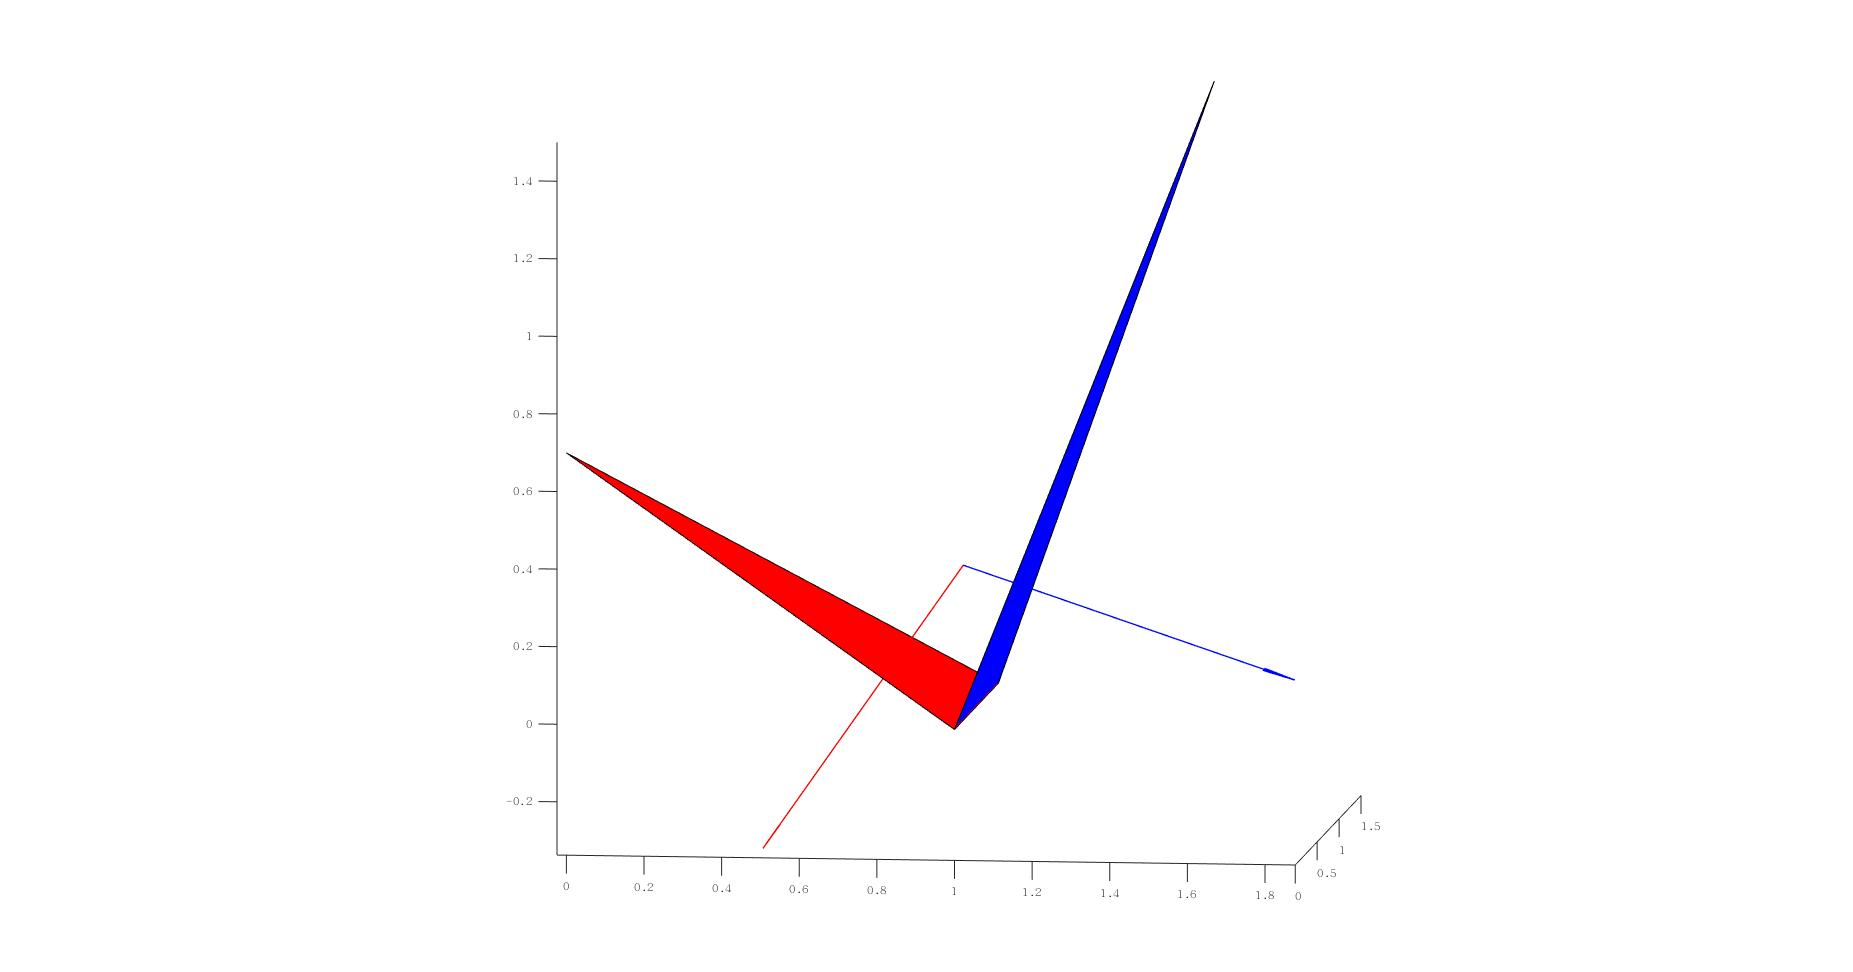
\includegraphics[width = .6\textwidth]{fig/s3p2.jpg}
        % \column{0.4\linewidth}<1->
        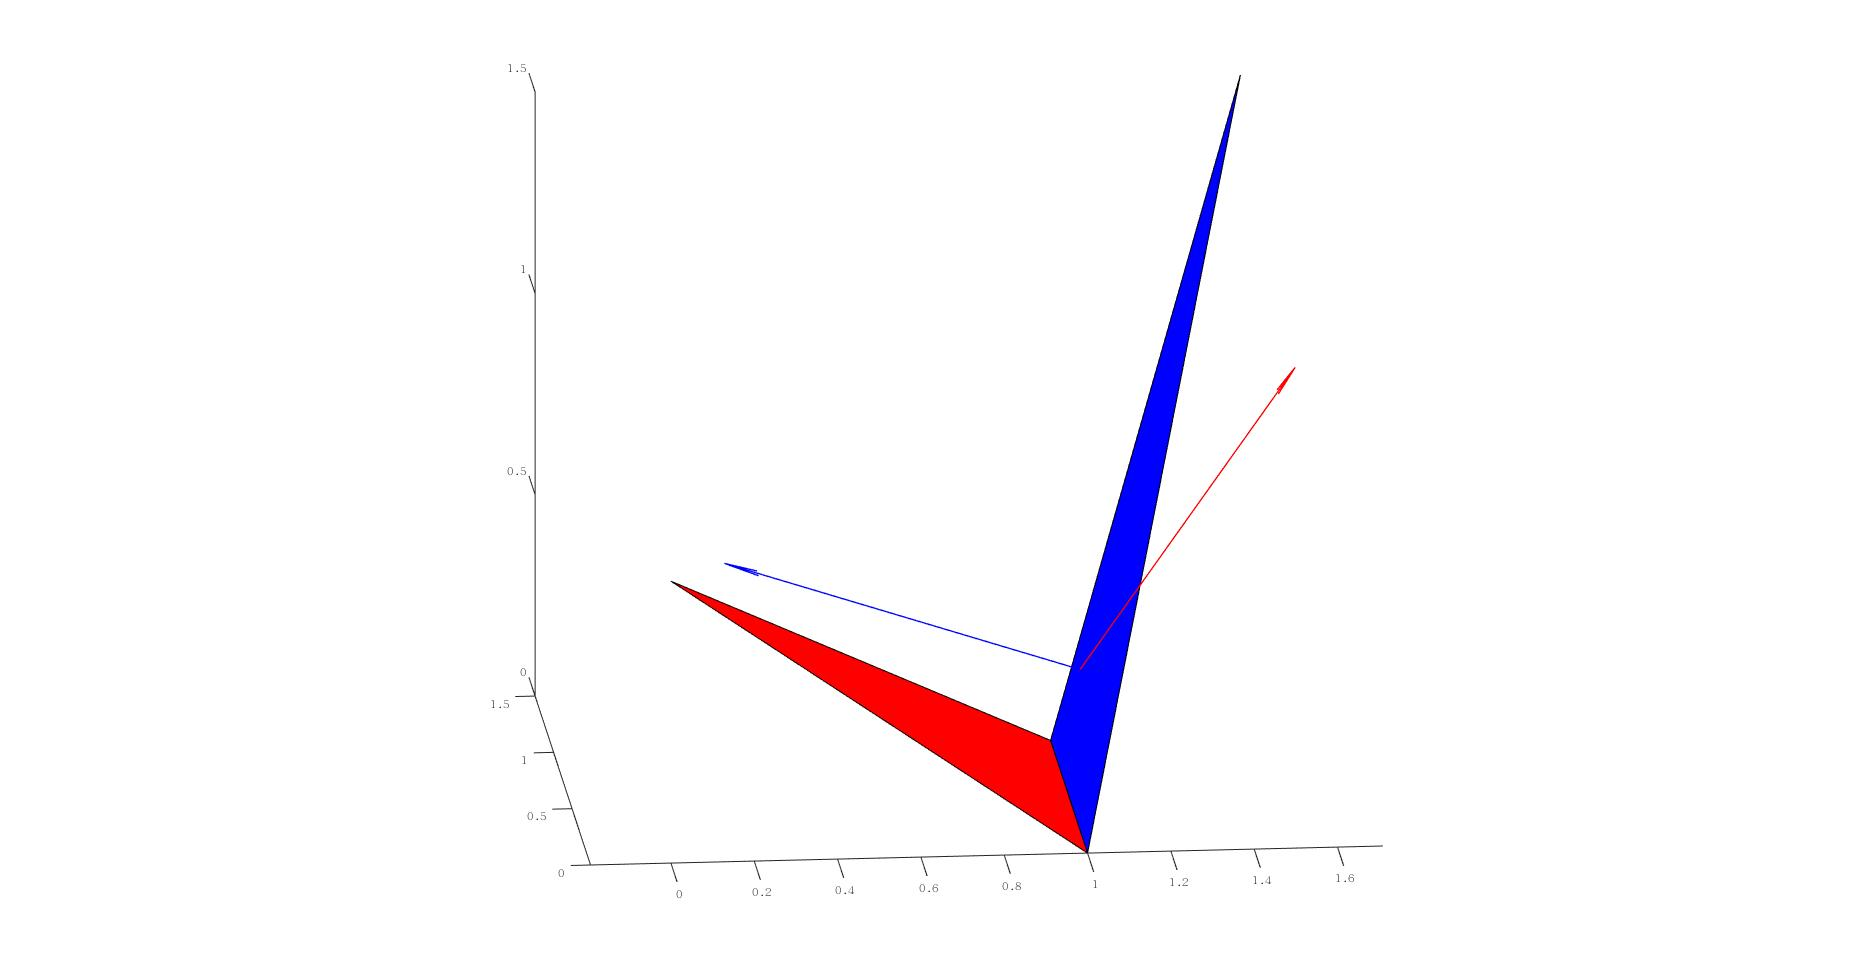
\includegraphics[width = .6\textwidth]{fig/s3p3.jpg}
        % \end{columns}
    \end{emt}
\end{frame}

\begin{frame}
    \begin{emt}[布尔运算的实现]
        \begin{enumerate}
            \setlength{\itemsep}{30pt}
            \item \textbf{求反运算 : } 转换曲面片的法向量方向,重新粘合曲面片(改变方向时好配对会变化).
            \item \textbf{求交运算 : } 移除不在另一个殷集内部的曲面片,然后粘合剩余的曲面片.
            \item \textbf{求并运算 : } 分别求反后求交,再求反得并集.
        \end{enumerate}
    \end{emt}
\end{frame}

\section{攻读博士学位的规划}

\begin{frame}
    \frametitle{海洋内波的理论 \caesura 模型与计算.}
    \begin{emt}[原理\cite{wangzhan_1589}]
        \begin{itemize}
            \item 盐度与温度在垂直方向上的差异造成海水的密度分层现象.
            \item 当内部扰动或外部影响造成等密面波动的现象被称为海洋内波.
            \item 海洋内波在全球范围普遍存在,并且在海峡入海口等密度分层现象长时间
            存在的区域会有频繁的内波活动.
        \end{itemize}
    \end{emt}

    \begin{emt}[首次研究\cite{npg-18-193-2011}]
        \begin{itemize}
            \item V. W. Ekman是第一个详细研究死水现象起源的研究者.他博士时期
            相关工作的动机来自挪威北极探险家的记录良好的报告.Fridtjof Nansen               
            1893年在"Nordeskiold"群岛附近遭遇了这种现象.

            \item 他通过使用不同类型的船在双层流体上演化,
            对这一现象的几个方面进行了描述.
        \end{itemize}
    \end{emt}
\end{frame}

\begin{frame}
    \begin{emt}[死水实验\cite{npg-18-193-2011}]
        2011年为纪念Nansen 船长诞辰150周年, 法国里昂高等师范学院物理实验室的
        Matthieu Mercier等实验流体力学家利用现代实验手段复现了Ekman的死水实验.
        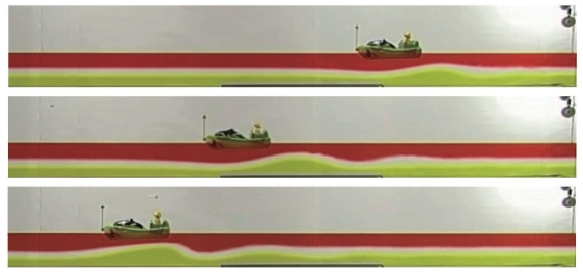
\includegraphics[width = \textwidth]{fig/s4p1.png}
    \end{emt}
\end{frame}

\begin{frame}
    \begin{emt}[意义\cite{wangzhan_1589}]
        \begin{itemize}
            \item 潜艇湍流尾迹的海洋表面特征等内波现象的研究,用于潜艇追踪和隐身.
            \item 还能直接应用于内波对各种海洋结构物和部件(平台、立管、锚链等)的作用力计算,
            是进一步分析海洋结构物的响应、强度和疲劳的前提和基础.
            对于我国的海洋工程尤其是深海油气资源的开发具有重要的意义
        \end{itemize}
        
    \end{emt}
    
\end{frame}

\begin{frame}
    \bibliographystyle{amsalpha}

\bibliography{bib/cas-refs}
\end{frame}

\begin{frame}
    \begin{center}
        \Huge 感谢老师们的倾听!
    \end{center}
\end{frame}


% \end{CJK}
\end{document}